\section{Homepage}
In this section the homepage will be analyzed from the point of view of the usability. 
Since many components of the website are "shared" across different pages (they are the same even in internal pages), this section will contain also the analysis of the shared ones.

\subsection{Informative Axes}
The informative axes (6w) should provide the users with all the fundamental information regarding the website. 
If users are not able to collect those information, they are not willing to stay and navigate through the website, since they are not getting the information that they want.

\begin{figure}[h!]
	\centering
	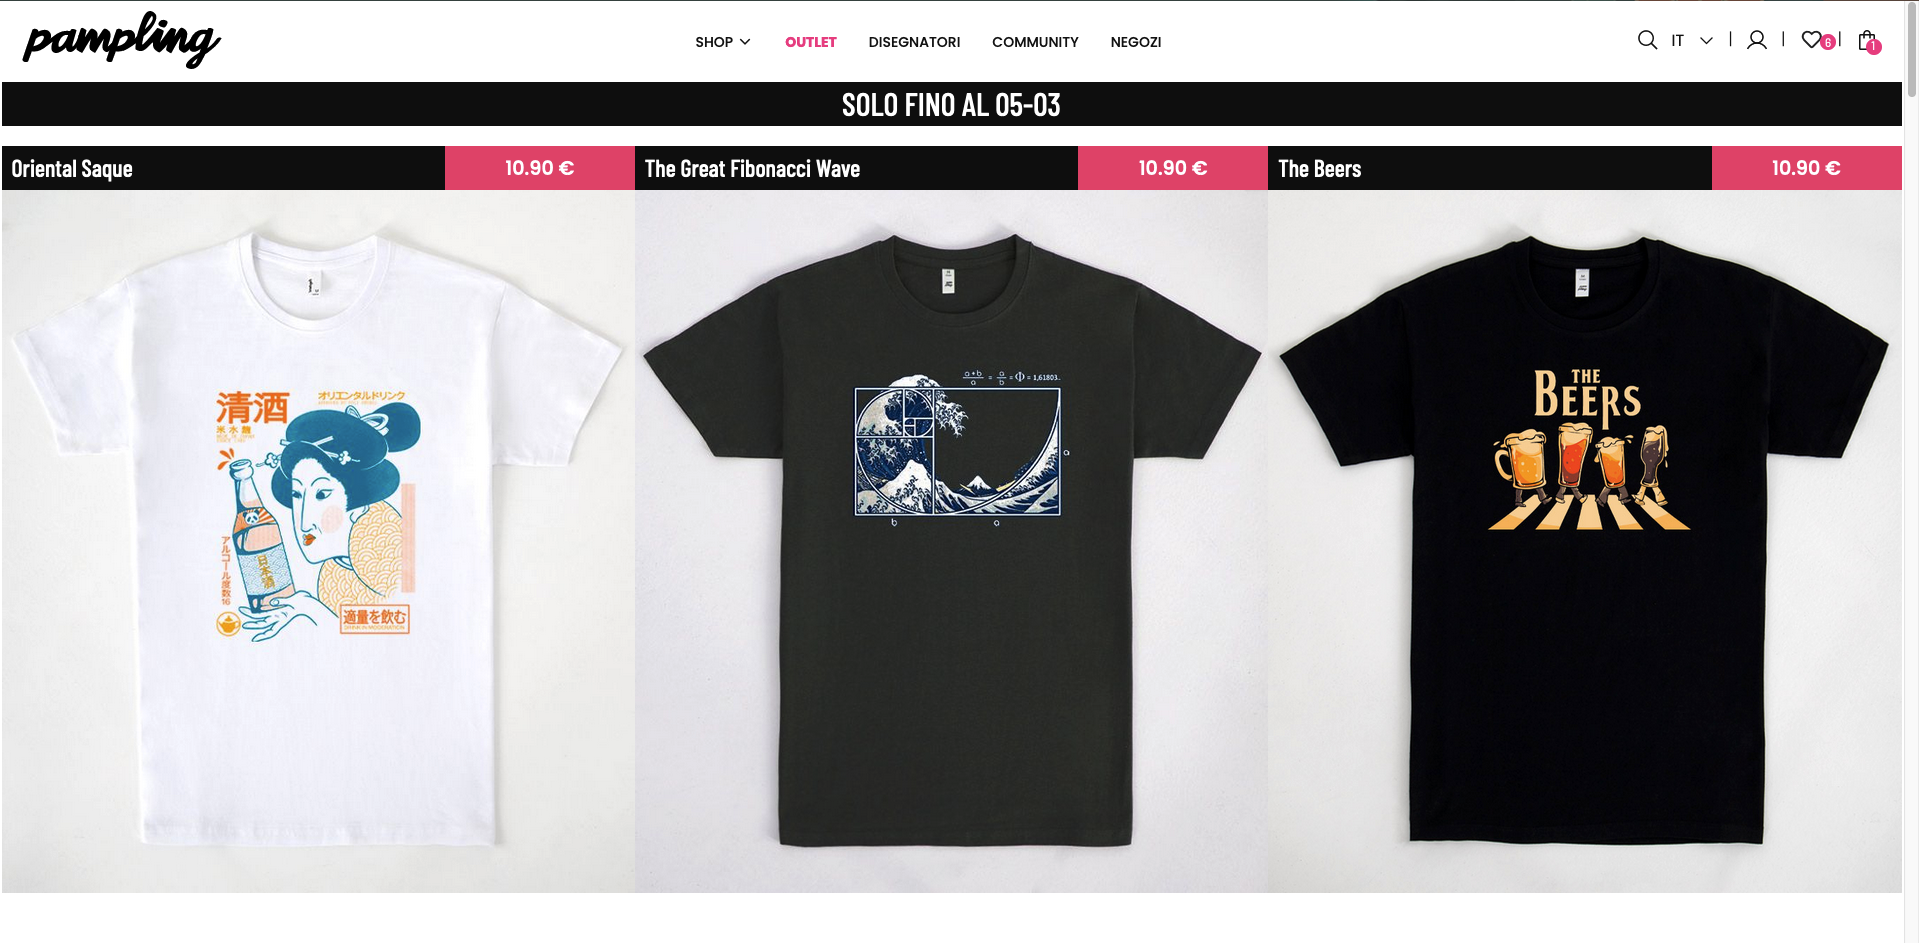
\includegraphics[scale=0.225]{images/homepage-first.png}
	\caption{homepage at first visit.}
	\label{fig:homepage-first}
\end{figure}

\subsubsection{WHERE did the user arrive?}
The website should give all the available information to the users regarding their relative position in the website, as well as a general idea about it. \\

If the where axis is not there, the user may experience the "lost in navigation" problem, which may lead to anger and frustration.\\
On the homepage of the website a complete menu of the website can be seen, that allows to reach all the possible pages of the website. 
On the top left corner of the homepage, in a standard position, there is the logo that links to the homepage.
The fact that the logo can be found in a standard position is a good choice, as the user will always be able to find it
and will be also able to find easily his way out of an unkown place.\\ 
Navigating through the website pages the breadcrumbs appear (of type "Location", which shows the absolute path from the website's root up to the specific page).
Not all the internal pages have them though, and this is not a good choice since it may lead to user confusion.
Another element that may confuse the user, in particular if there are no breadcrumbs present, is the face that in the menu the page "Outlet" is always in a 
different font with respect to the other pages (bold and of a different color). This might bring users to think that they are currently in that section of the 
website even if it is not true.

\subsubsection{WHO is behind the website?} 
The "who" axis should give the information about the website's owner.\\

Again, the logo in the top-left corner is really good to immediately understand the owner of the website. 
A good characteristic of the logo is that it is verbal and not just an image. 
A negative side is that the is no slogan of any kind: in this way, a user that arrives on the website without knowledge about this company
will not have many information about them.
In oder to get more information about the authors, the user is forced to scroll until the very end of the homepage. 
There he will find the footer (\cref{fig:footer}) where there may seem to be a link to a section of the website which aims to describe the company ("About Pampling").\\
Actually, if the user clicks there, the page shown is a FAQ page that does not give any information about the company.
Beacuse all of the points above, the "who" axis is not really satisfied and new users will have difficulties in understanding who's behind the site.

\begin{figure}[h!]
	\centering
	
\includegraphics[scale=0.225]{images/footer.png}
	\caption{footer of the website.}
	\label{fig:footer}
\end{figure}


\subsubsection{WHY should the user stay?} 
The "why" axis should provide motivations to users to persuade them to stay and navigate within the website.\\

The homepage without scrolling shows some offers currently active, that may catch the user attention and give a motivation to navigate further the website and that's positive.
On the other hand, the fact that these offers occupy the whole visible part of the homepage is not totally good, since it requires some scroll to the user to reach other content
that might be of better used if positioned at the start of the page.
For example, scrolling down (approximatively 1.5 scrolls) some \textit{catch phrases} are found that give some motivations for the user to stay in the website.
Examples in \cref{fig:slogan}.\\
The average user is not willing to scroll that much in the homepage, that is why putting \textit{catch content} that down (talking about scrolling) may not capture the users' attention.

\begin{figure}[h!]
	\centering
	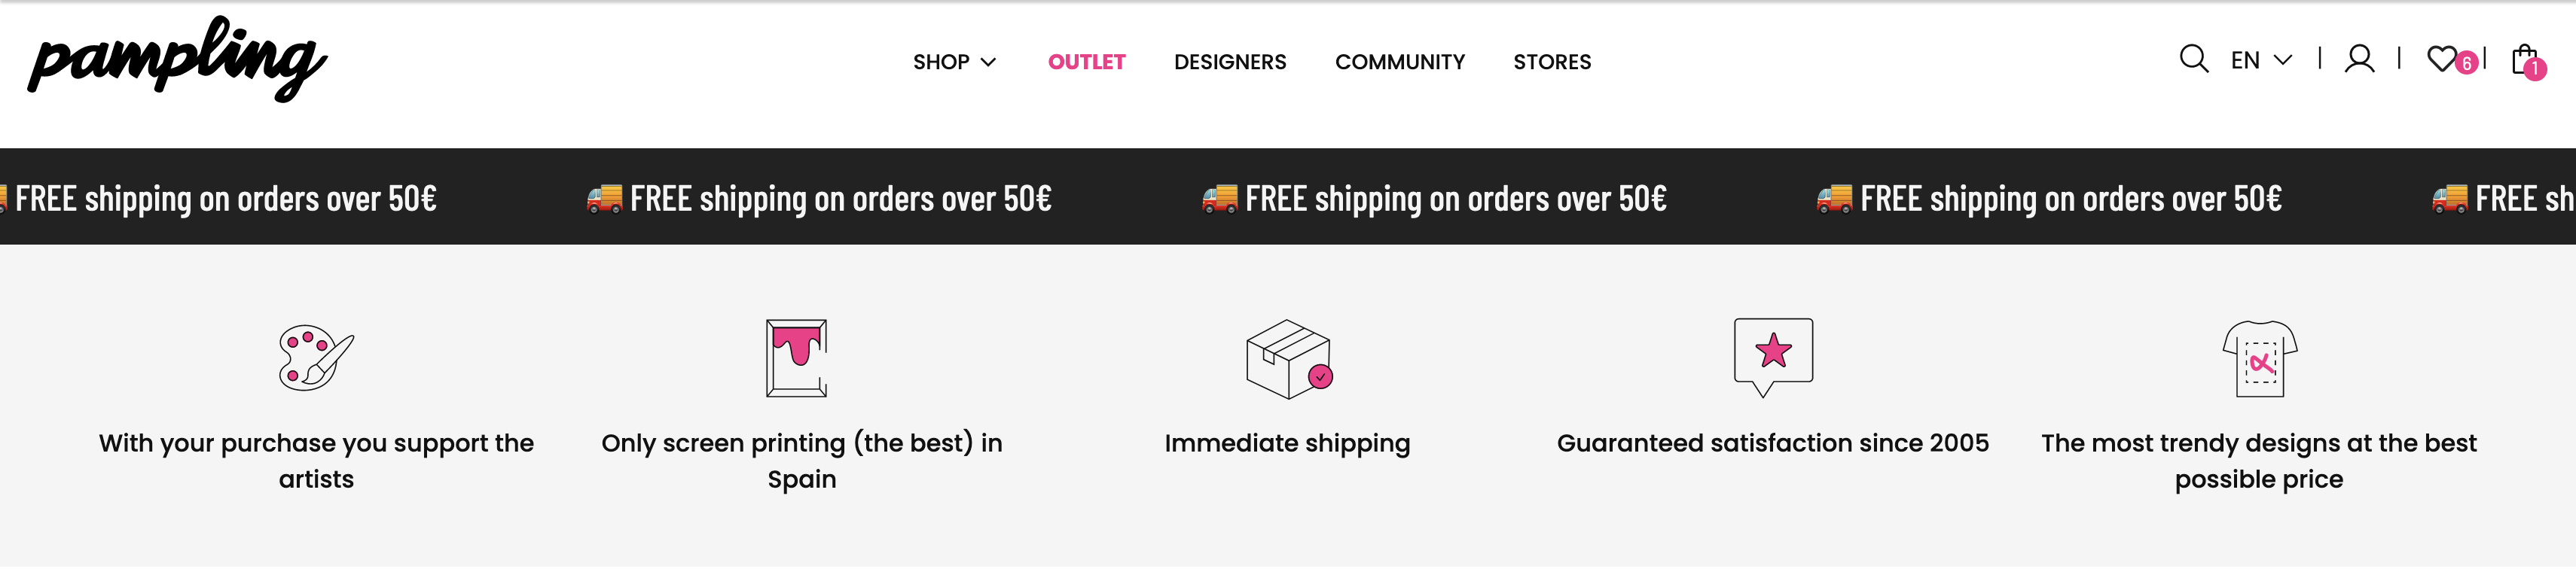
\includegraphics[scale=0.225]{images/slogan.png}
	\caption{slogans on the homepage.}
	\label{fig:slogan}
\end{figure}

\subsubsection{WHAT choices does the user have?} 
Another important axis is the "what" one. It should give the users access to all the possible destinations of the website.\\

As said before, there is a menu placed right at the beginning of the homepage (\cref{fig:homepage-first}).  
The menu is always the same even in internal pages: that's a really good choice in order to avoid possible confusion of the user and allow easy and quick navigation.
The menu will be better analyzed in a later section of this document.


\subsubsection{WHEN (latest news)} 
This axis should provide to the users all the latest news regarding the products and the company.\\

The first thing the user sees when entering the website are the latest discounts and promotions that make the user understand that the site is updated and active.
Furthermore, the website offers a "Community" section where the user can access and interact with all the latest news and articles created by other users or by Pampling itself.
In particular there are two different sections: the Pampling blog (\cref{fig:blog-pamplig}) and the Users blog (\cref{fig:blog-users})
Given these points, the "when" axis is quite satisfied.

\begin{figure}[h!]
	\centering
	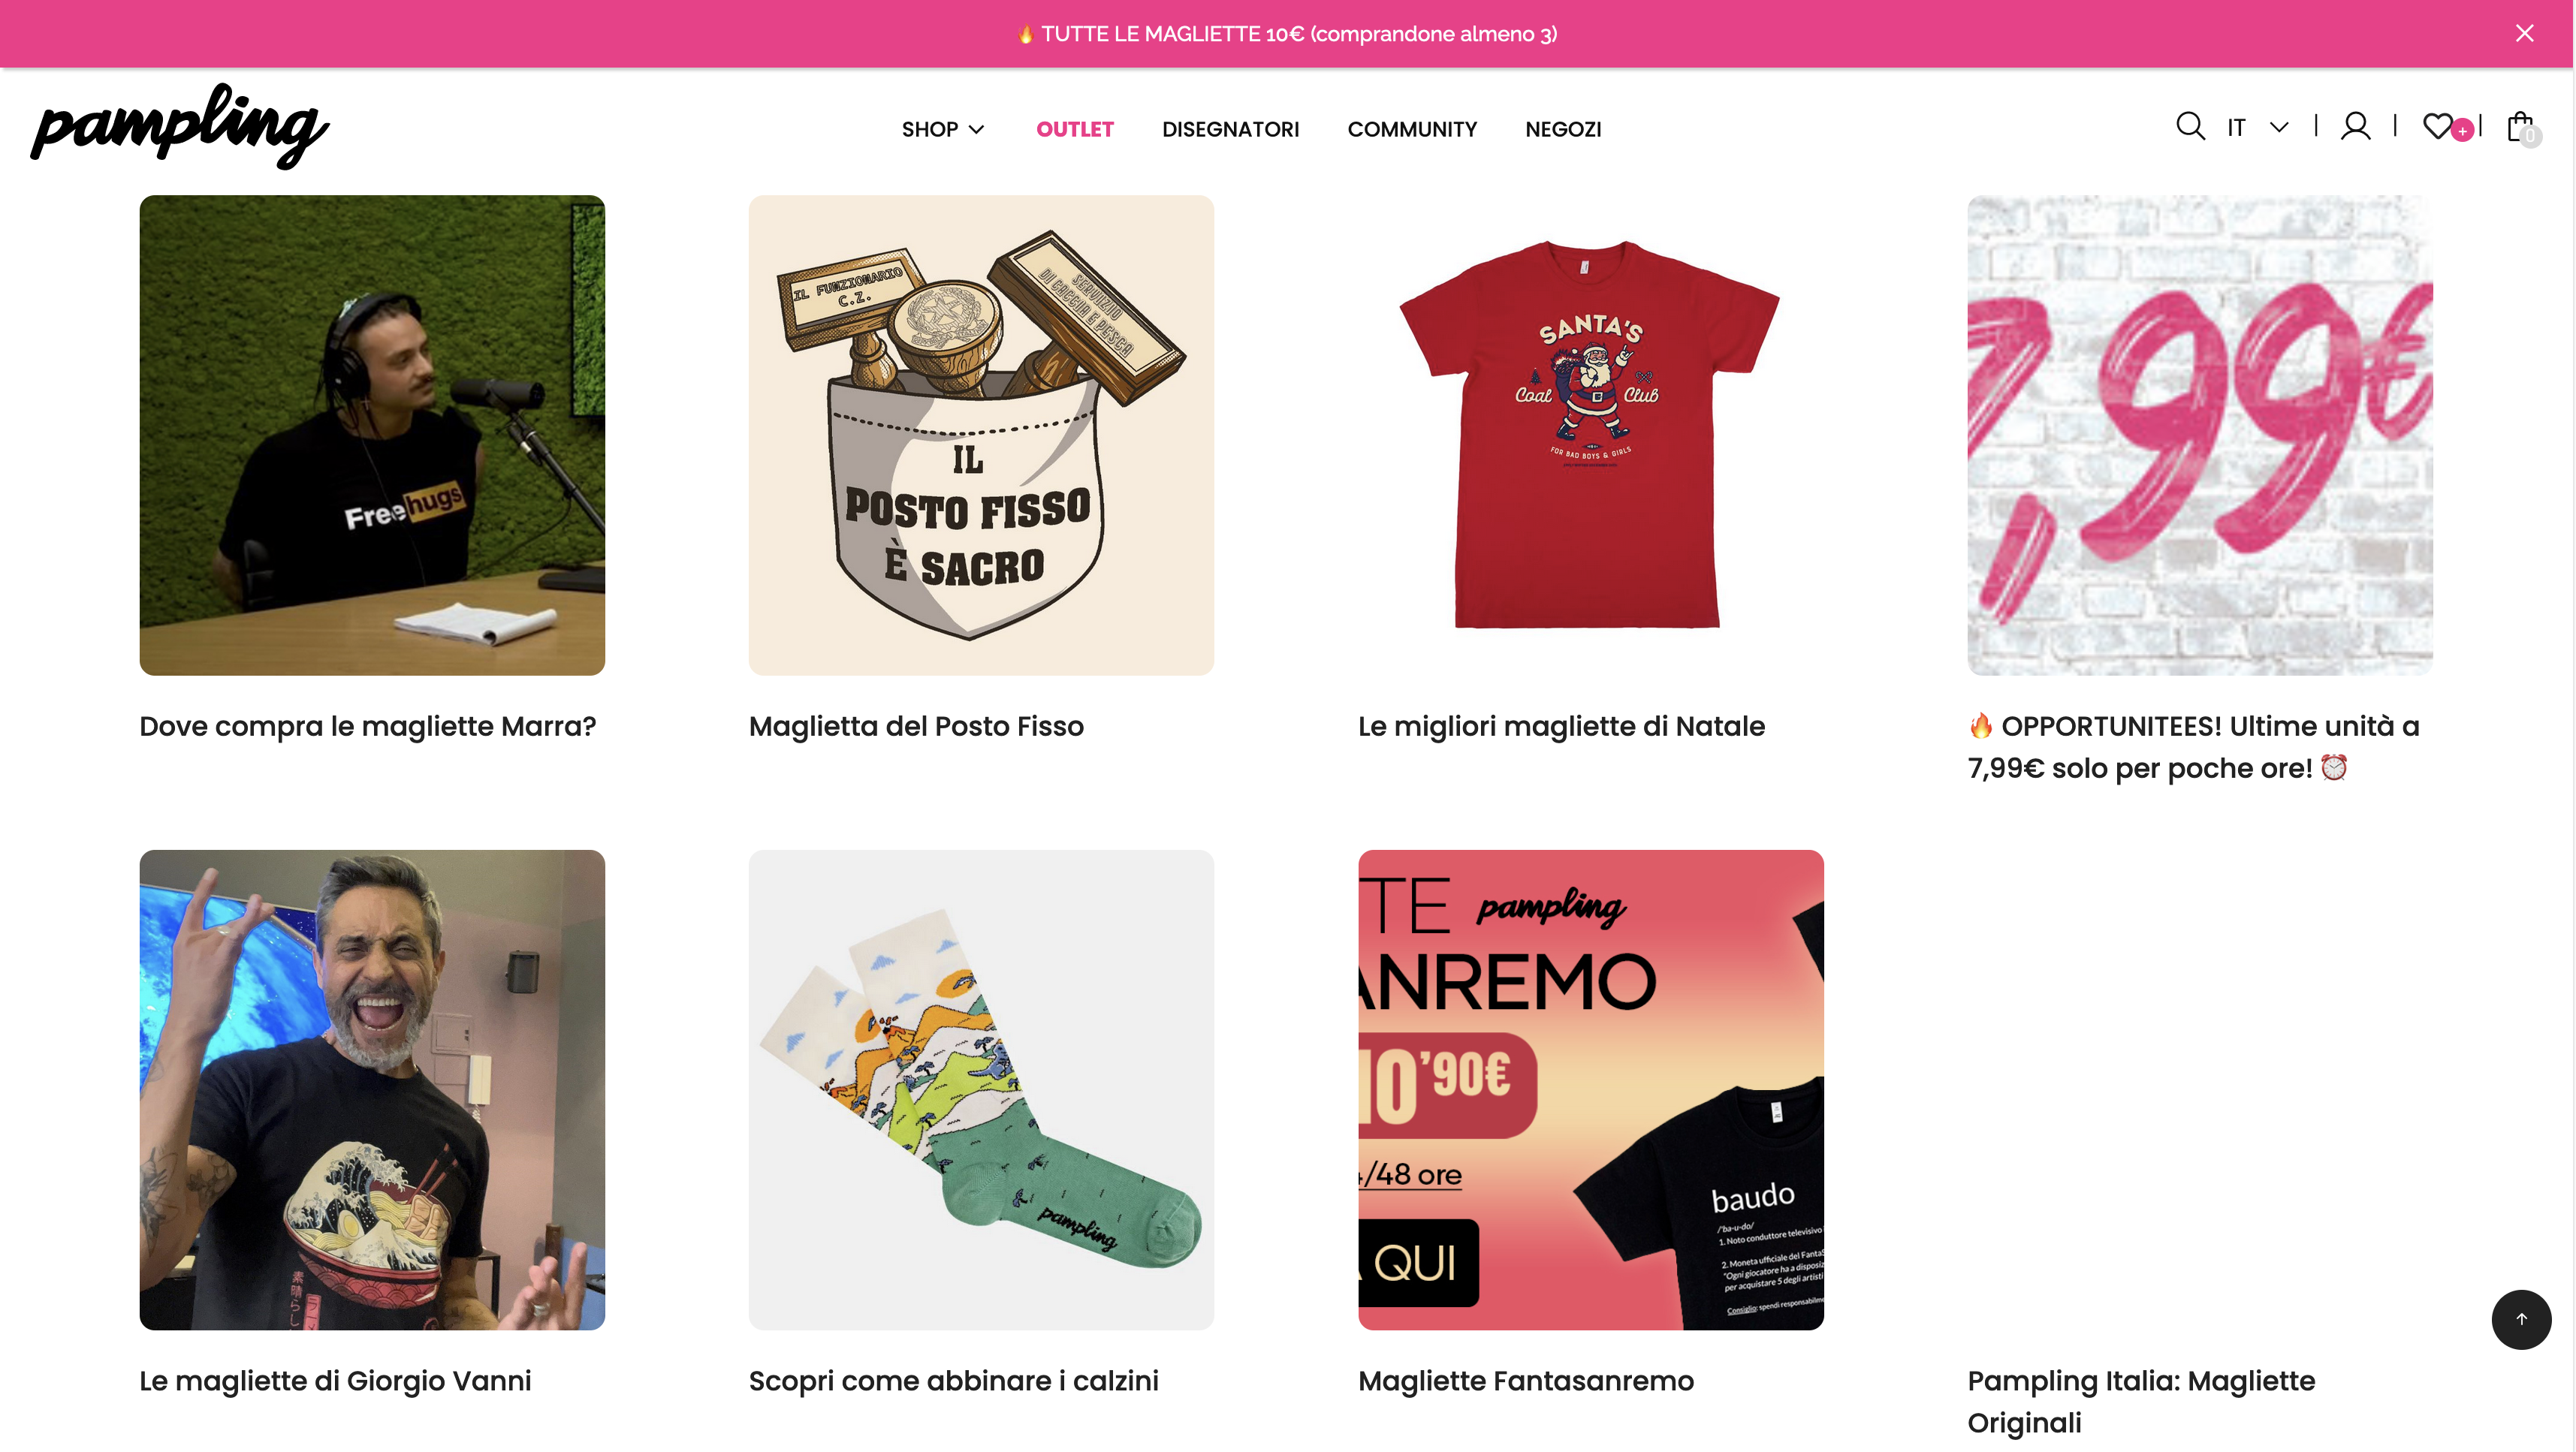
\includegraphics[scale=0.225]{images/blog-pampling.png}
	\caption{Pampling blog.}
	\label{fig:blog-pampling}
\end{figure}

\begin{figure}[h!]
	\centering
	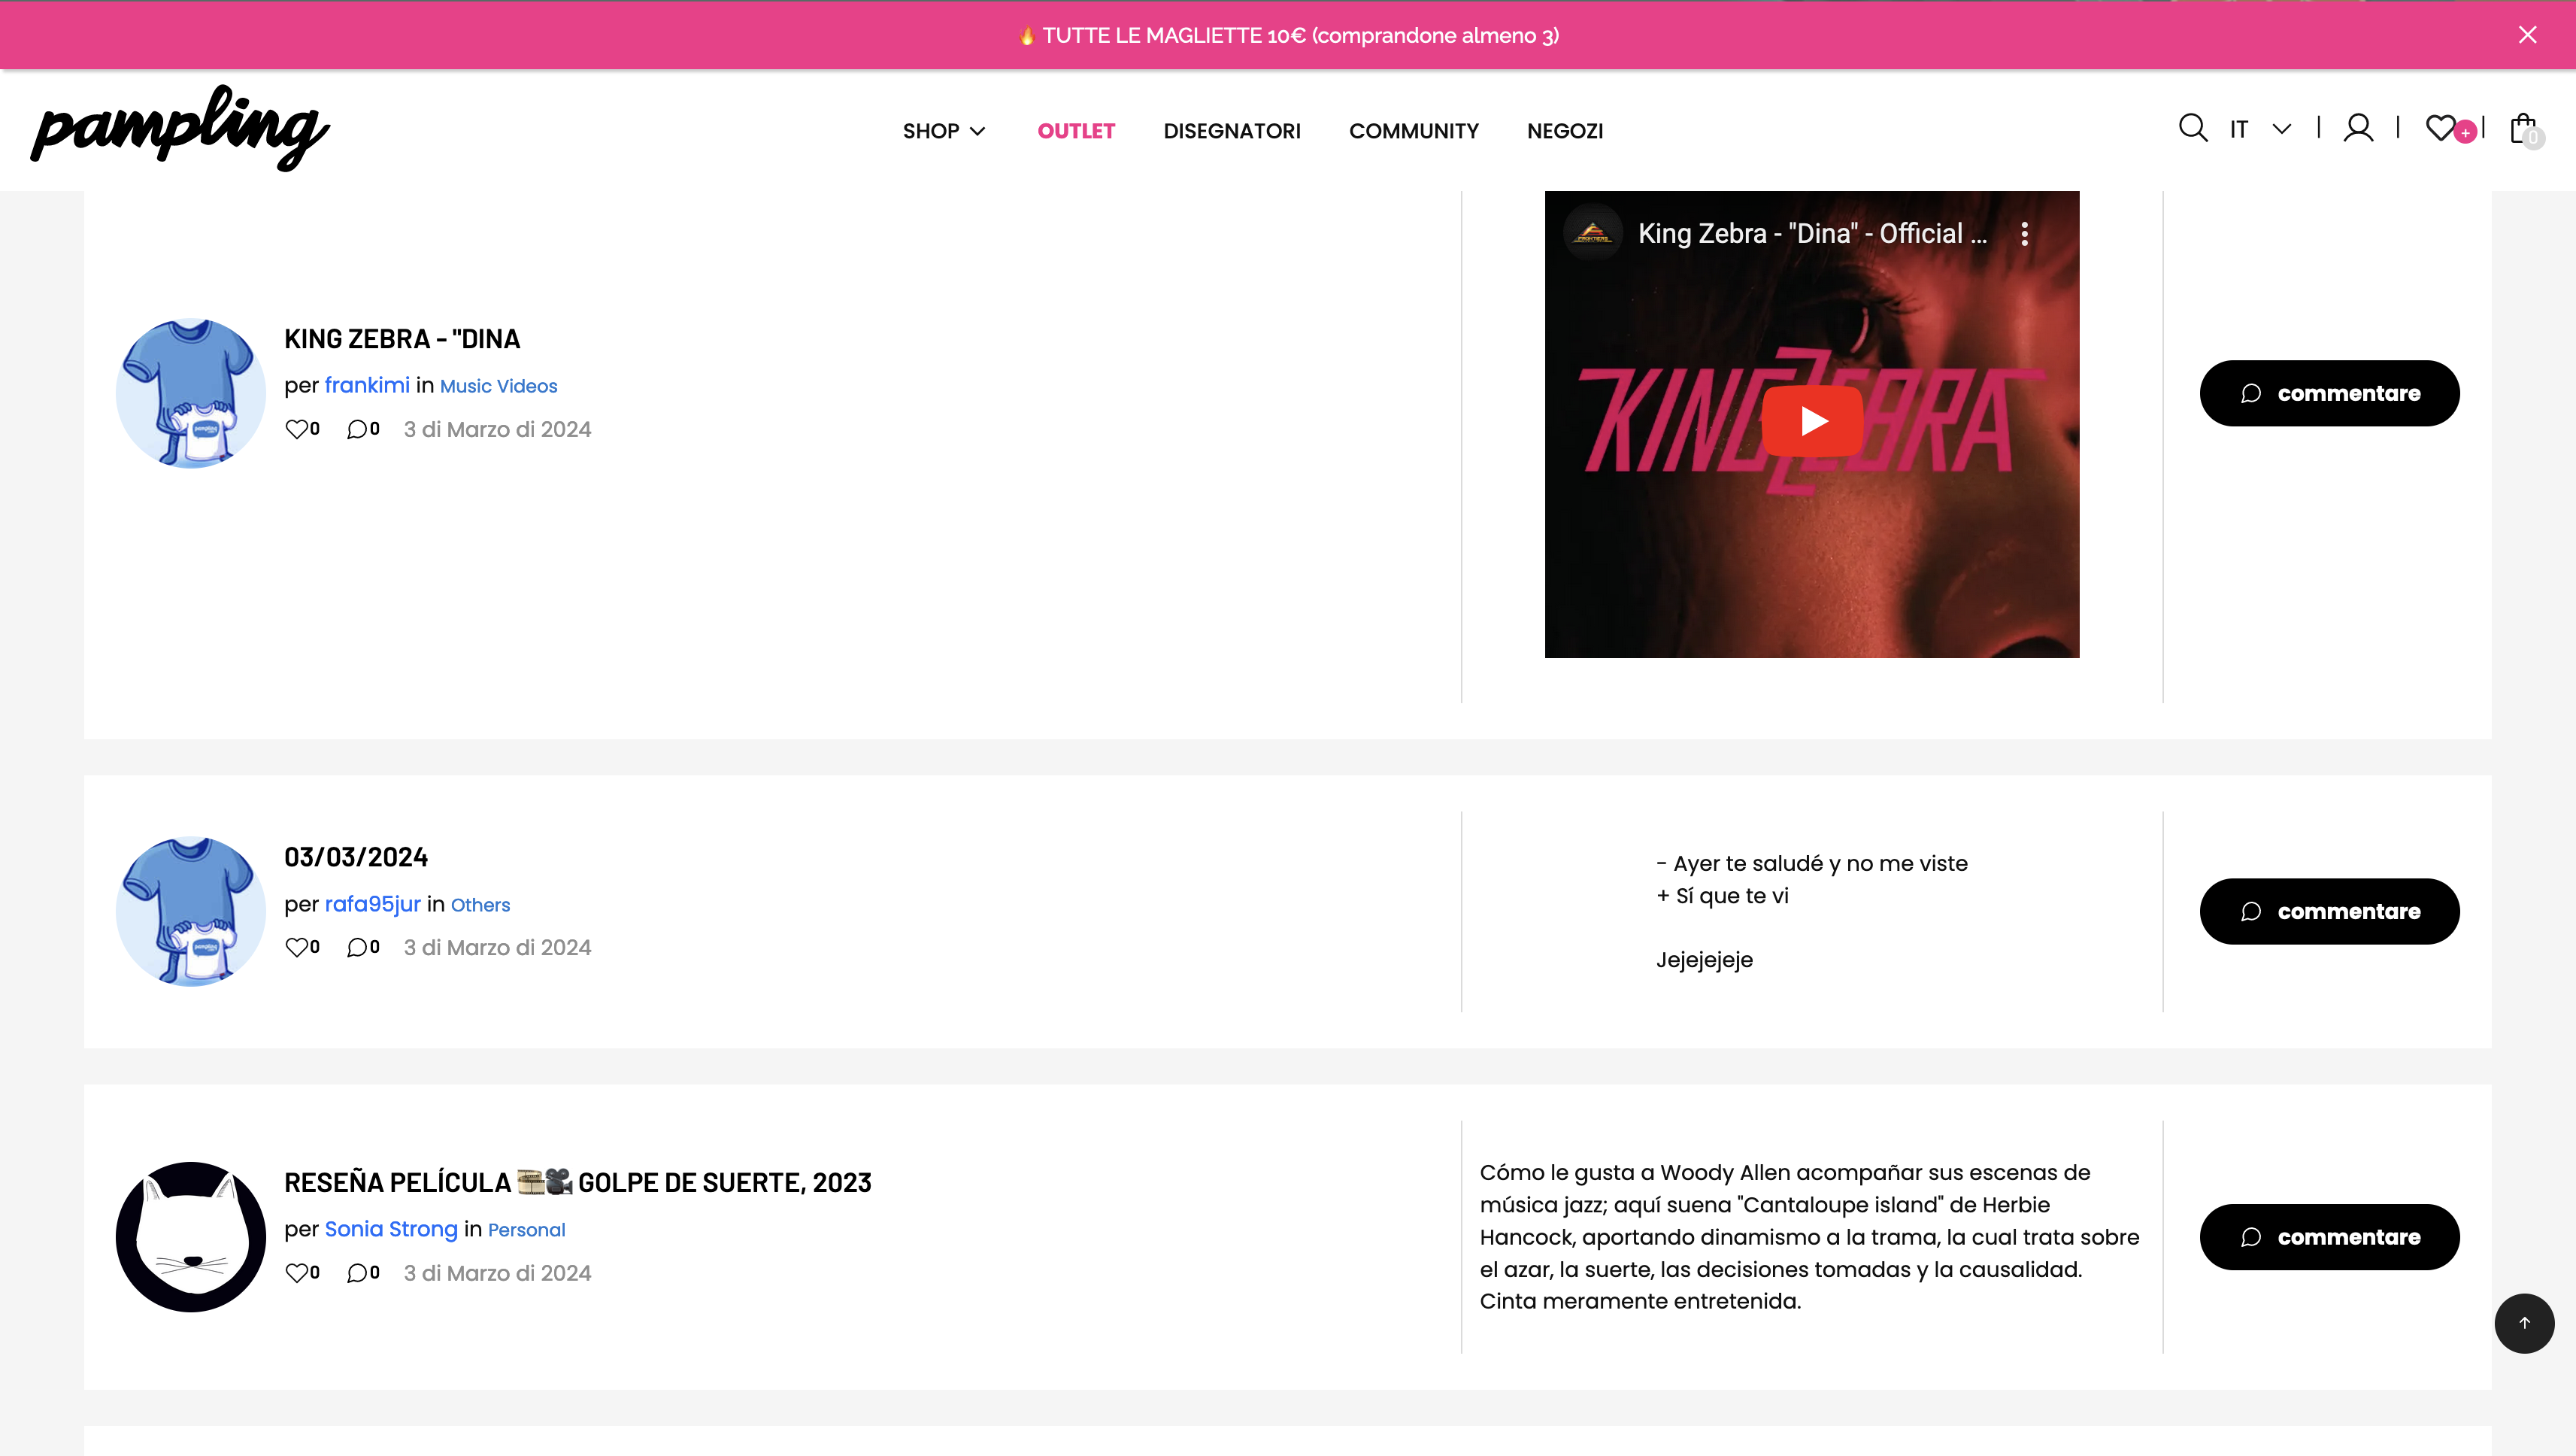
\includegraphics[scale=0.225]{images/blog-users.png}
	\caption{Users blog.}
	\label{fig:blog-users}
\end{figure}


\subsubsection{HOW to arrive where the user wants?} 
The axis should offer tools to the users in order to let them access and collect information in a smart way.\\

Within the menu a search icon is available, which when clicked opens the search functionality. That is really good and fundamental for a website of this kind: it allows the user 
to directly search for what he's looking for without having to navigate through blindly through the whole website.\\
Moreover, the "Shop" voice in the menu is quite complete with all the categories of products that are available for purchase: this allows the user to find what he needs even if he has 
only a general idea.


\subsection{Asking for Personal Data}
The website is freely accessible by everyone, with the possibility to create an account in case the user wants to purchase something 
or partecipate in the blogs offered by the website. 
A positive thing is that at the beginning of the visit there's no blocking pop-up asking for personal user data. 
At the end of the homepage the website offers the possibility to subscribe to the newsletter by giving the email address.
The placement is accetable since it is not blocking for any activity and is at the end of the page.
A random pop-up appears while scrolling the homepage the first time, as shown in \cref{fig:popup}. Since it is what it is (a popup), it is really annoying for the users. The only good thing about this negative situation, is that it can be easily removed and thus users are not required to fill it.


\subsection{Scrolling and Resolution}
\subsubsection{Scrolling}
Scrolling requires computational effort, that is why having too much scroll is bad. Typically users are willing to scroll up to 1.3 "screens" of a website page. Generally speaking, the quantity of scrolling may depend on the content of the page.\\

\paragraph{Vertical Scroll}
In order to see the entire homepage, the user is required to scroll a lot, at least 10 scrolls are required. 
Generally, users are not willing to do more than 1.3 scrolls on average and this indicates that the homepage is way too long.
It contains a lot of images and products that almost make it seems like another shop section.\\
There are different font measures and patterns in the disposition of the content that might overload the user.
Having so much scroll may lead the users to skip content of the page and thus they may miss important information.

\paragraph{Horizontal Scroll}
In the homepage there are also some parts that require horizontal scroll: this is not good since it requires more actions to the users
to access the information (two axis instead of one).

\subsubsection{Resolution}
The homepage, and generally speaking the website, seems to not suffer of the "frozen layout" problem. 
In fact, even if the resolution changes, the web site is adaptive and fit the screen entirely. 
The website offers also a mobile version for smaller resolutions.


\subsection{Menu}
The homepage (and website) menu can be seen on \cref{fig:menu}, where the biggest part of the dropdown menu is shown. 
The menu is one of the most important components of a website: it allows the user to navigate through it and 
also to discover all the pages and information that can be accessed within it.

\begin{figure}[h!]
	\centering
	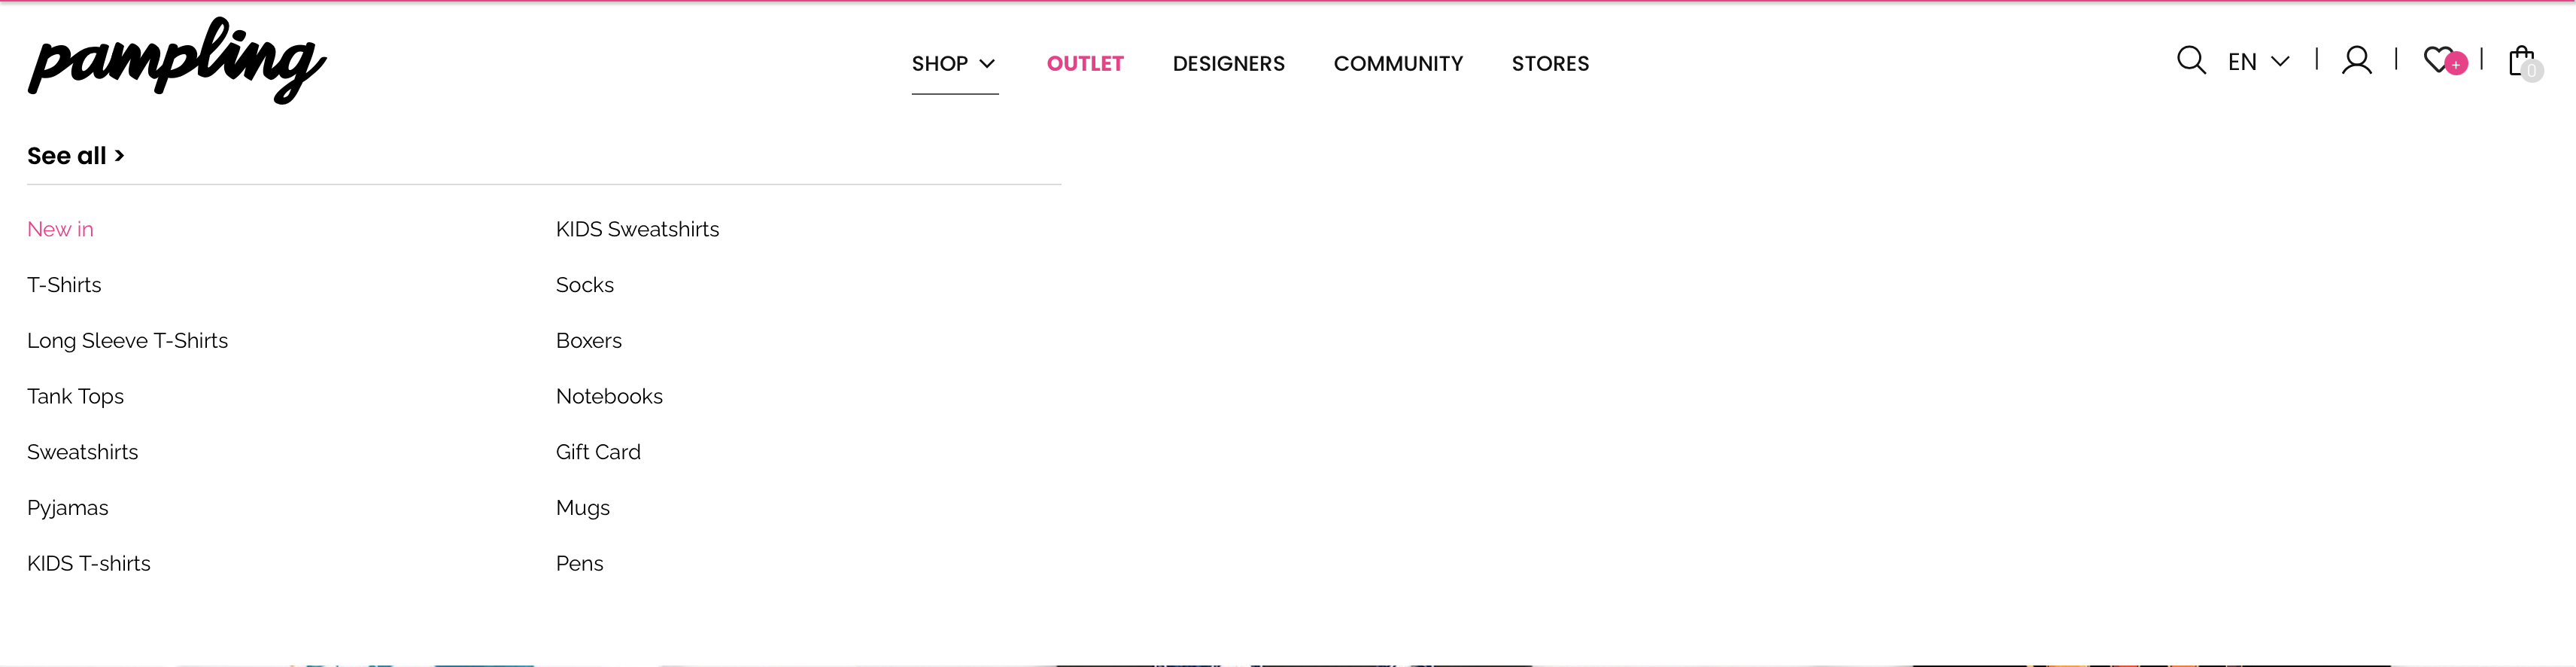
\includegraphics[scale=0.225]{images/menu.png}
	\caption{menu of the website}
	\label{fig:blog-users}
\end{figure}

The website's menu is a pretty common one. It is a horizontal menu with 5 entries. 
It has not a tree-like structure, since it is constructed on 2 informative levels only: the general one (first) and the detailed one (second, which shows all the options regarding a first-level entry)\\
The menu is a dropdown, a good choice to facilitate its use to the user since it's less prone to error in point-and-click operations. 
Because of this no fault-tolerance algorithm is required, since there is no possibility of having the menu to close when inside a first-level entry.\\
Overall the menu has been implemented in a good way, by avoiding all the common and annying problems of the classic websites' menus.

\subsection{Content}
In this section the style of the main content will be analyzed. 
The homepage doesn't contain much written text that can be found only in internal pages like for example 
the one shown in \cref{fig:content}.

\begin{figure}[h!]
	\centering
	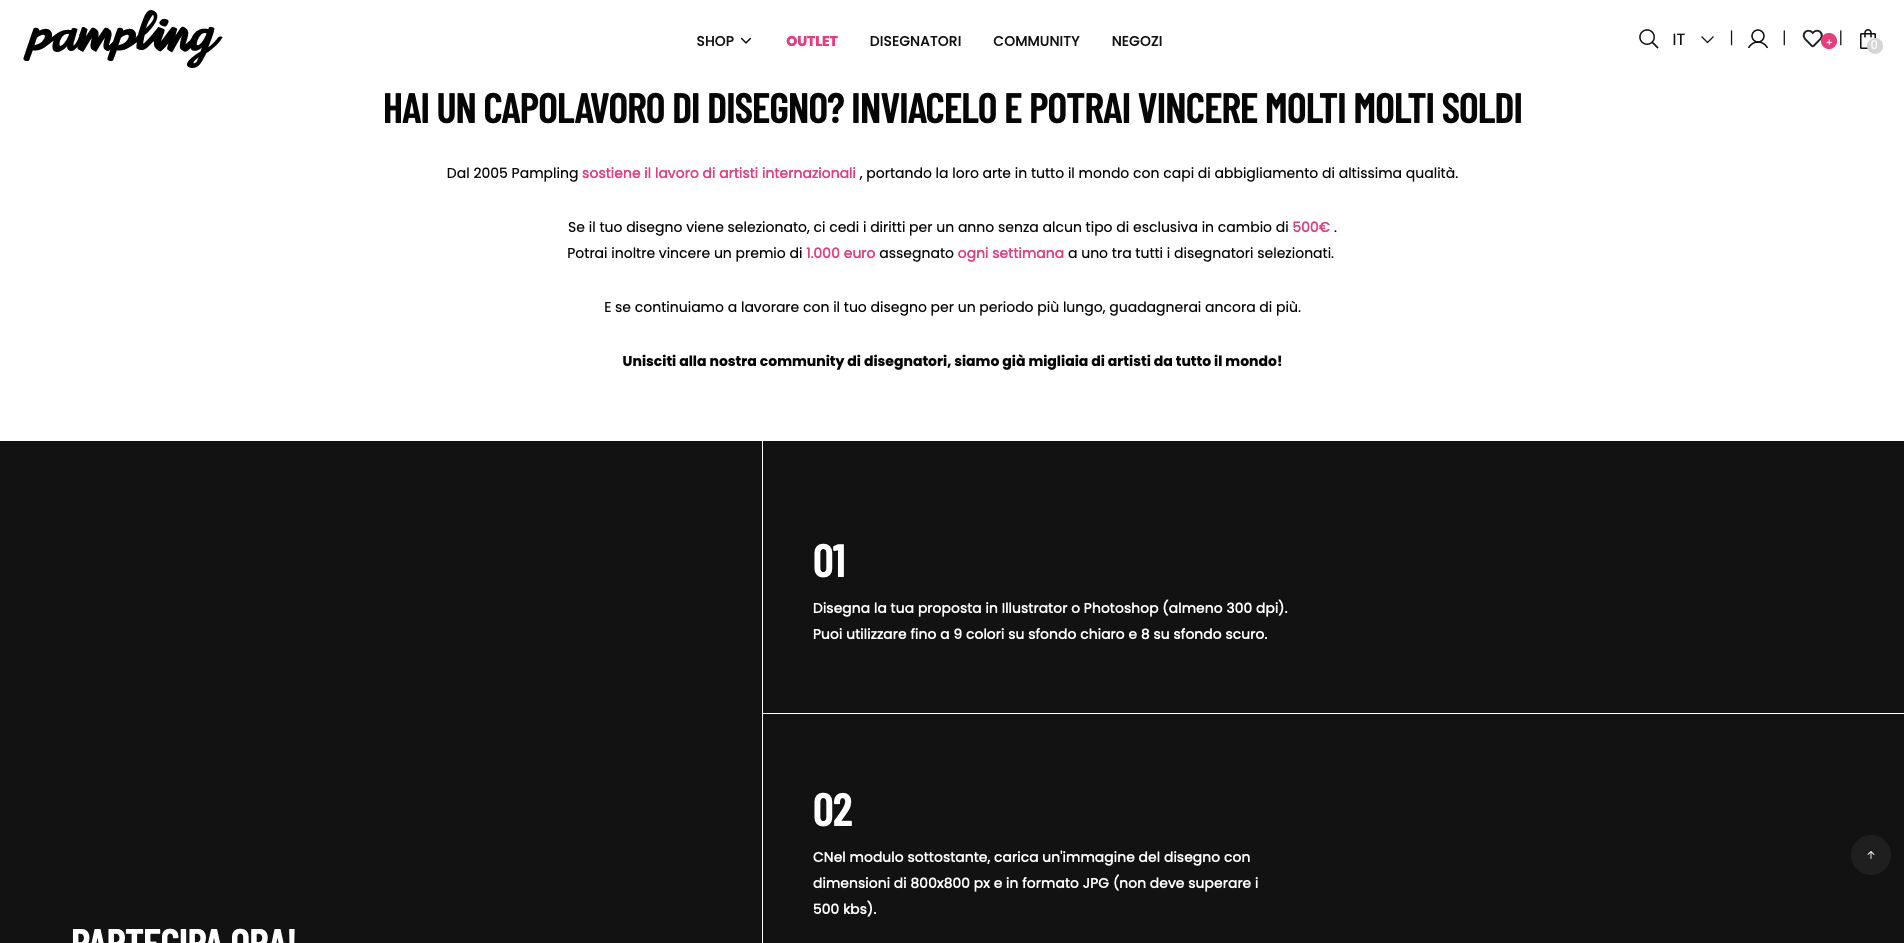
\includegraphics[scale=0.225]{images/content.png}
	\caption{menu of the website}
	\label{fig:content}
\end{figure}

\subsubsection{Text}
The text of the main content of the page must be readable. 
In order to achieve readability, a set of constraints must be respected.

\paragraph{Resizing Options}
There should be buttons (or even other ways) to allow the users to easily change the font size, without using zoom-in or zoom-out browser's tools.\\

The website is not offering resizing options. The only way to adjust the font size is by using the zoom functionality of the browser. 

\paragraph{Color and Font}
The font size is is right (about 13 or 14 points), bigger than the minimum 10 points required for readability. 
In addition, only one font is used within all the website, which is good choice.\\
Also the color of the text is well chosen since it's black on white background or white on black background. 
In general the readability is good.

\paragraph{Style}
A part from titles that are uppercase, the main text is lowercase. 
This is good since the user is not required to switch a lot between uppercase and lowercase while reading. 

\paragraph{Graphical Objects}
There is no text inside images, that is a good choice since text on images:
\begin{itemize}
\item Cannot be resized properly;
\item Will make the image to weight more, and thus more loading time;
\item Will make the "\textit{copy\&paste}" functionality to not work;
\item Will not be recognized by search engines that are crawling the webpage.
\end{itemize}


\subsubsection{Content Structure}
\paragraph{Structure}
As mentioned before, the homepage does not contain much written content, but mainly displays informations about current discounts
and offers.
Regarding other pages, the written content is still not much and the paragraphs are all quite short. 
The content looks like to be well structured and it does not seem to suffer of the "\textit{Lorem Ipsum}" 
problem (\textit{layout-design-first} problem). \\

\paragraph{Keywords}
The keyword are enlighted with a bold font or a different color that still has a good contrast with the background.\\
This is good because in this way the user will immediatly find the most important information within the page.

\paragraph{Lists}
Lists are really liked by users, since they help them to sumarize the information available on the content.

There are multiple lists inside the pages with the most written content. Some of them are good, as they contain
at least 4 items. \\
On the other hand, some other lists are not as good since sometimes they contain just one element. 
Moreover, there's a page (\href{https://www.pampling.com/}{Designers/Special content by Pampling}) that is 
entirely composed by lists: this may lead to a decrease of user satisfaction as too many lists require too much computational
effort to the user.

\subsection{Attention Map}
For the user to be able to see the crucial aspects of the website, it is importat to structure the content in a way that let
them capture the fundamental components of the webpage instantly.

\subsubsection{F-shape Map}
The \textit{F-shape} Map of attention is the way our eyes move while reading content in web pages. Thus, the most important 
components of the webpage should be placed within the top center of the webpage. \\
In the website, the \textit{F-shape} map is kept into consideration since the menu is placed in the best 
position possible, on the top of the page. Also the search button, the shopping cart, the button to change language 
and the user profile are in the top right of the page, the most common position for this kind of functionalities: 
This is a good choice because in this way users will find them easily. 
The homepage though requires a lot of scroll and contains a lot of big images (\textit{bloated design}), choice that partially 
vanishes the effect of the \textit{F-shape} attention map.

\subsubsection{Images}
While in a web page text is the most important component, images are also quite valuable. 
They can integrate the normal content, even if they tend to be skimmed.
The website is quite full of images. \\
Since images tend to attract clicks, in general is better to associate an action to every click event on an image.
This is quite respected within the website since the majority of the images are clickable redirect the user to another page, 
like the product or a search-by-category page.

\subsection{Searching}
Even if the website is not big (and thus a search functionality is not strictly required from a theoretical point of view),
the search functionality is present. I think that in a website of this kind, with the great amount of fandoms and topics referred by
the clothing products, the search tool is almost a neccessary functionality. 

\subsubsection{Search Tools}
The search functionality can be activated by clicking on the lens icon, placed near the top-right corner.


\subparagraph{No Result}
\begin{figure}[h!]
	\centering
	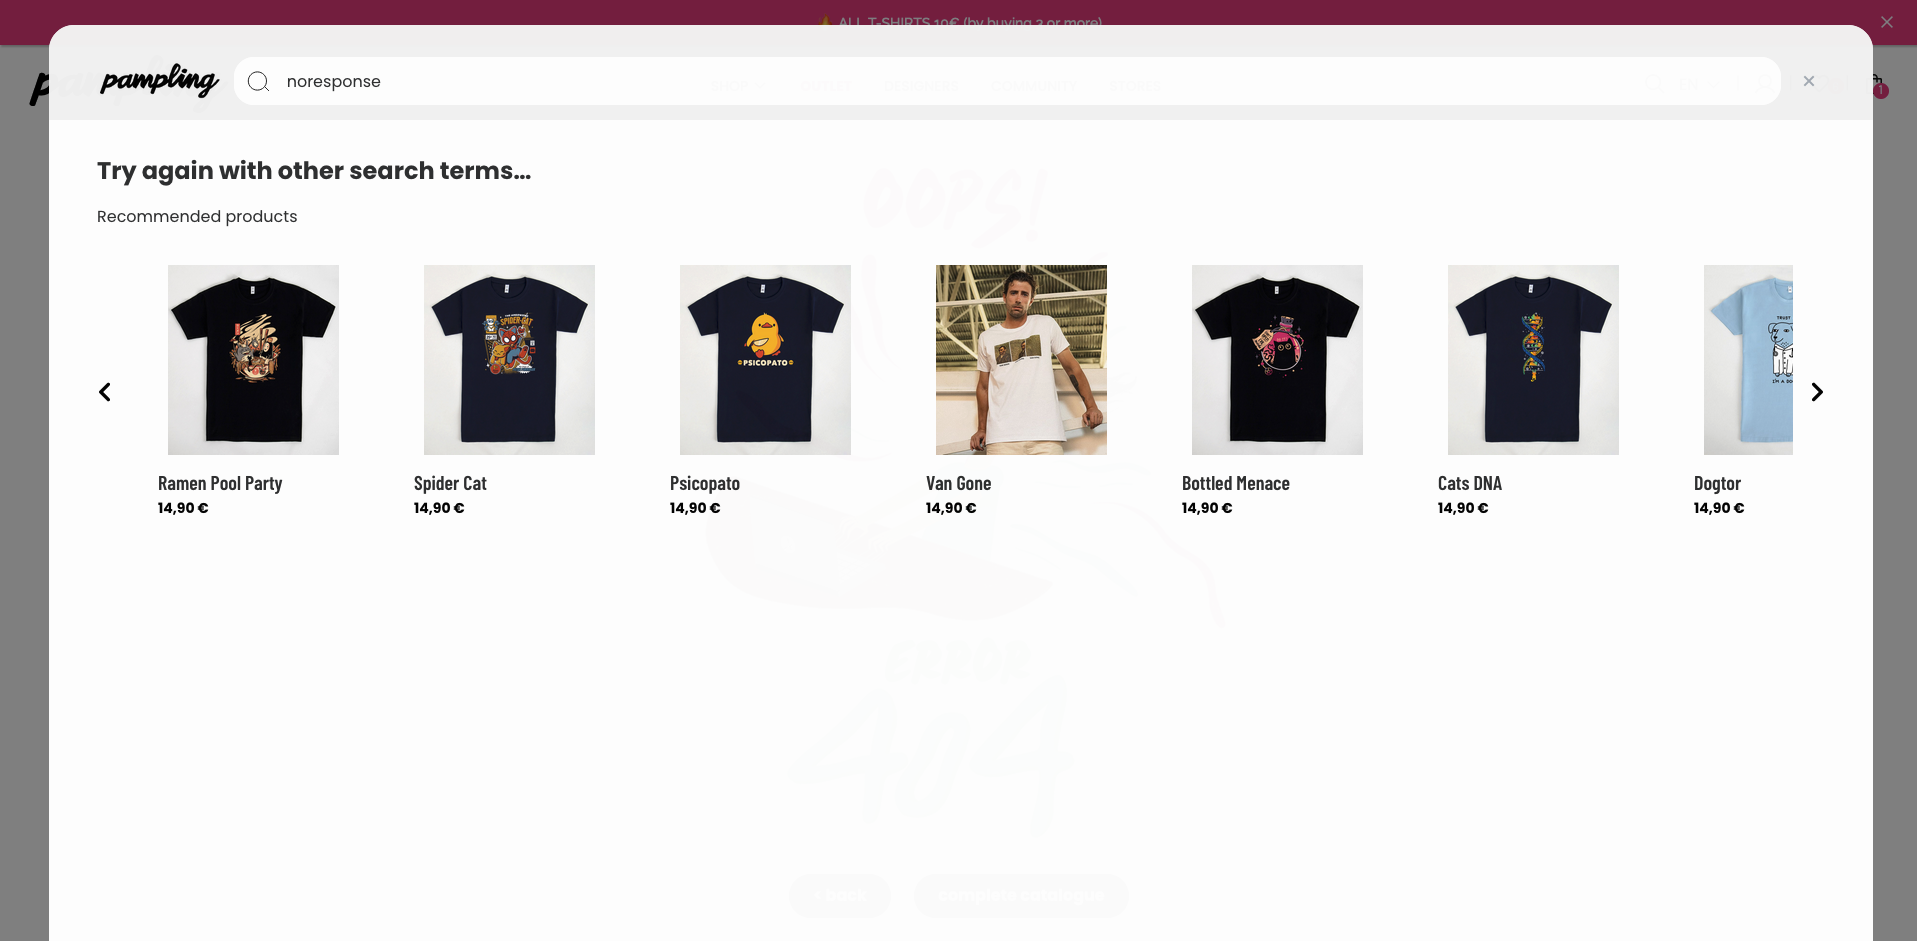
\includegraphics[scale=0.225]{images/zero-res.png}
	\caption{no result webpage.}
	\label{fig:zero-res}
\end{figure}

\begin{figure}[h!]
	\centering
	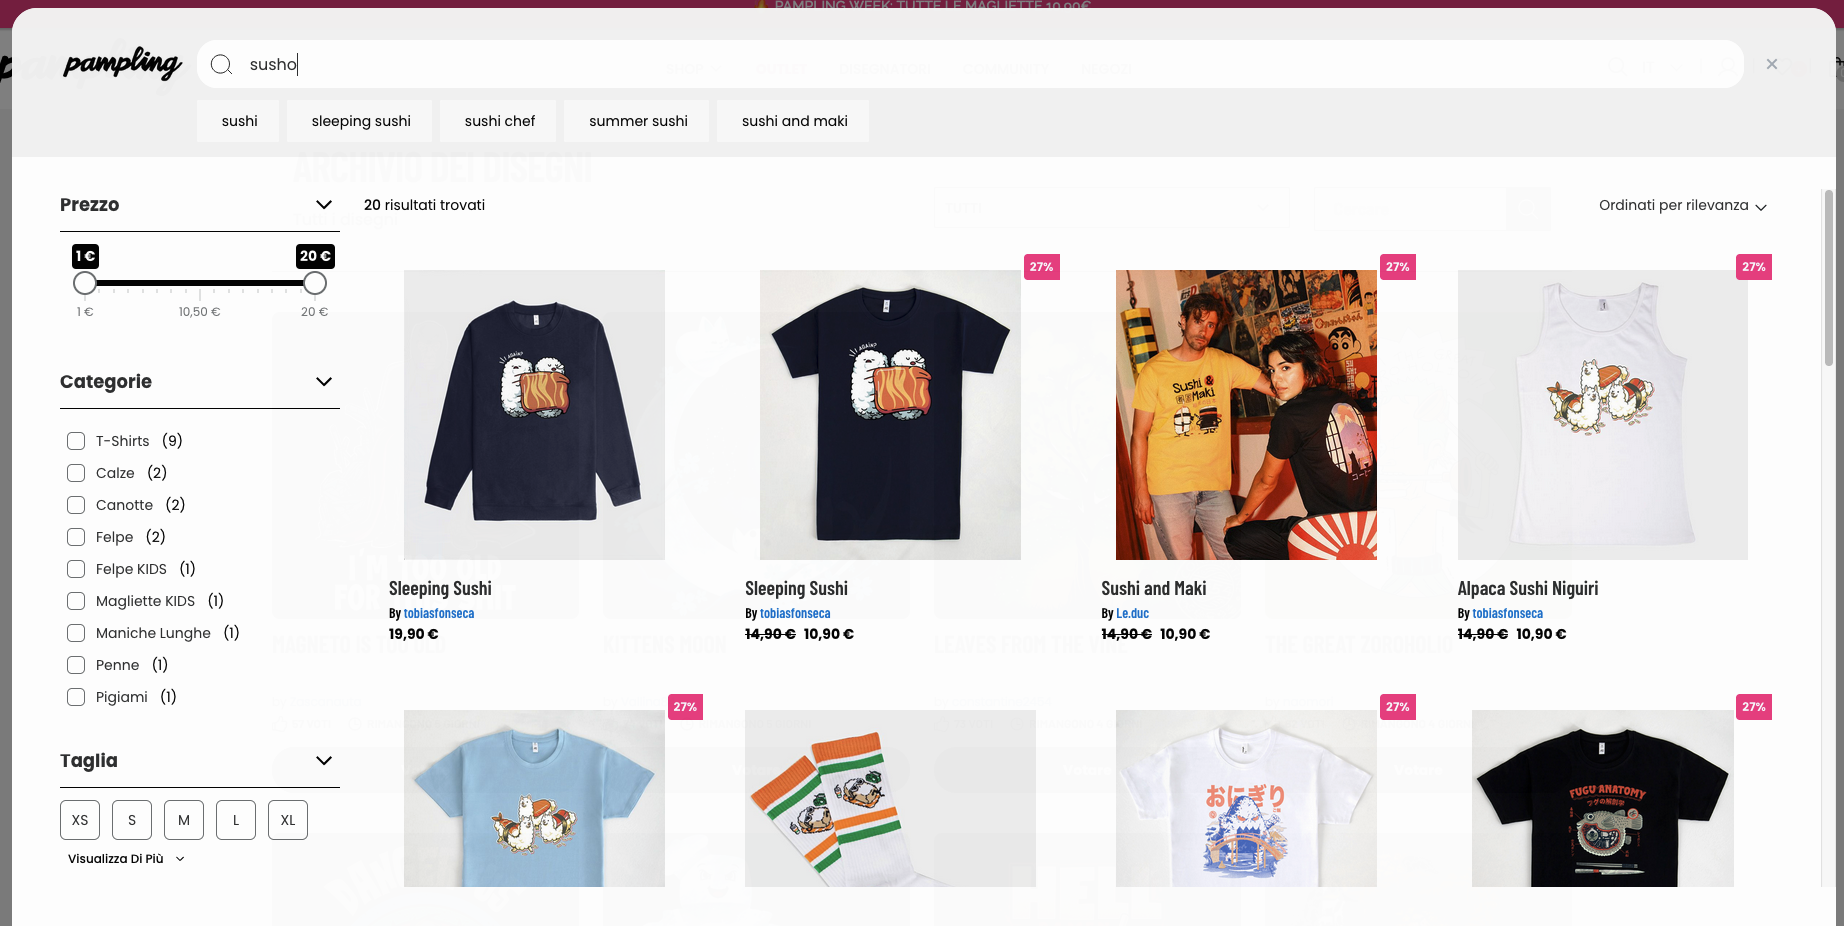
\includegraphics[scale=0.225]{images/wrong-search.png}
	\caption{wrong keyword search.}
	\label{fig:wrong-search}
\end{figure}

The screen in \cref{fig:zero-res} is the result when looking for keywords that return no results.
The way in which the website handles it is good: even if the searched keyword is not relevant, some other products are shown
to the user in order to help him navigate further and find other article that might be of their interest.

Moreover, the search is dealing well even with typos, since it still show articles that are actually coherent with the 
intended keyword. An example can be seen in \cref{fig:wrong-search}.

\cref{fig:wrong-search} shows also that filters are present here in the search panel, which is good to 
help the user to get to their objective faster.
Once the user has found what they're looking for, by clicking on the product, the related product page opens.

\subsubsection{Search Box}
The length of users' queries increased a lot in past years, as a result of having much more information available on the web.
The search bar in the website is quite large, which invites the user to search for longer queries. This is good because 
the results will be more precise and the level of satisfaction of the user will be higher. 

\begin{figure}[h!]
	\centering
	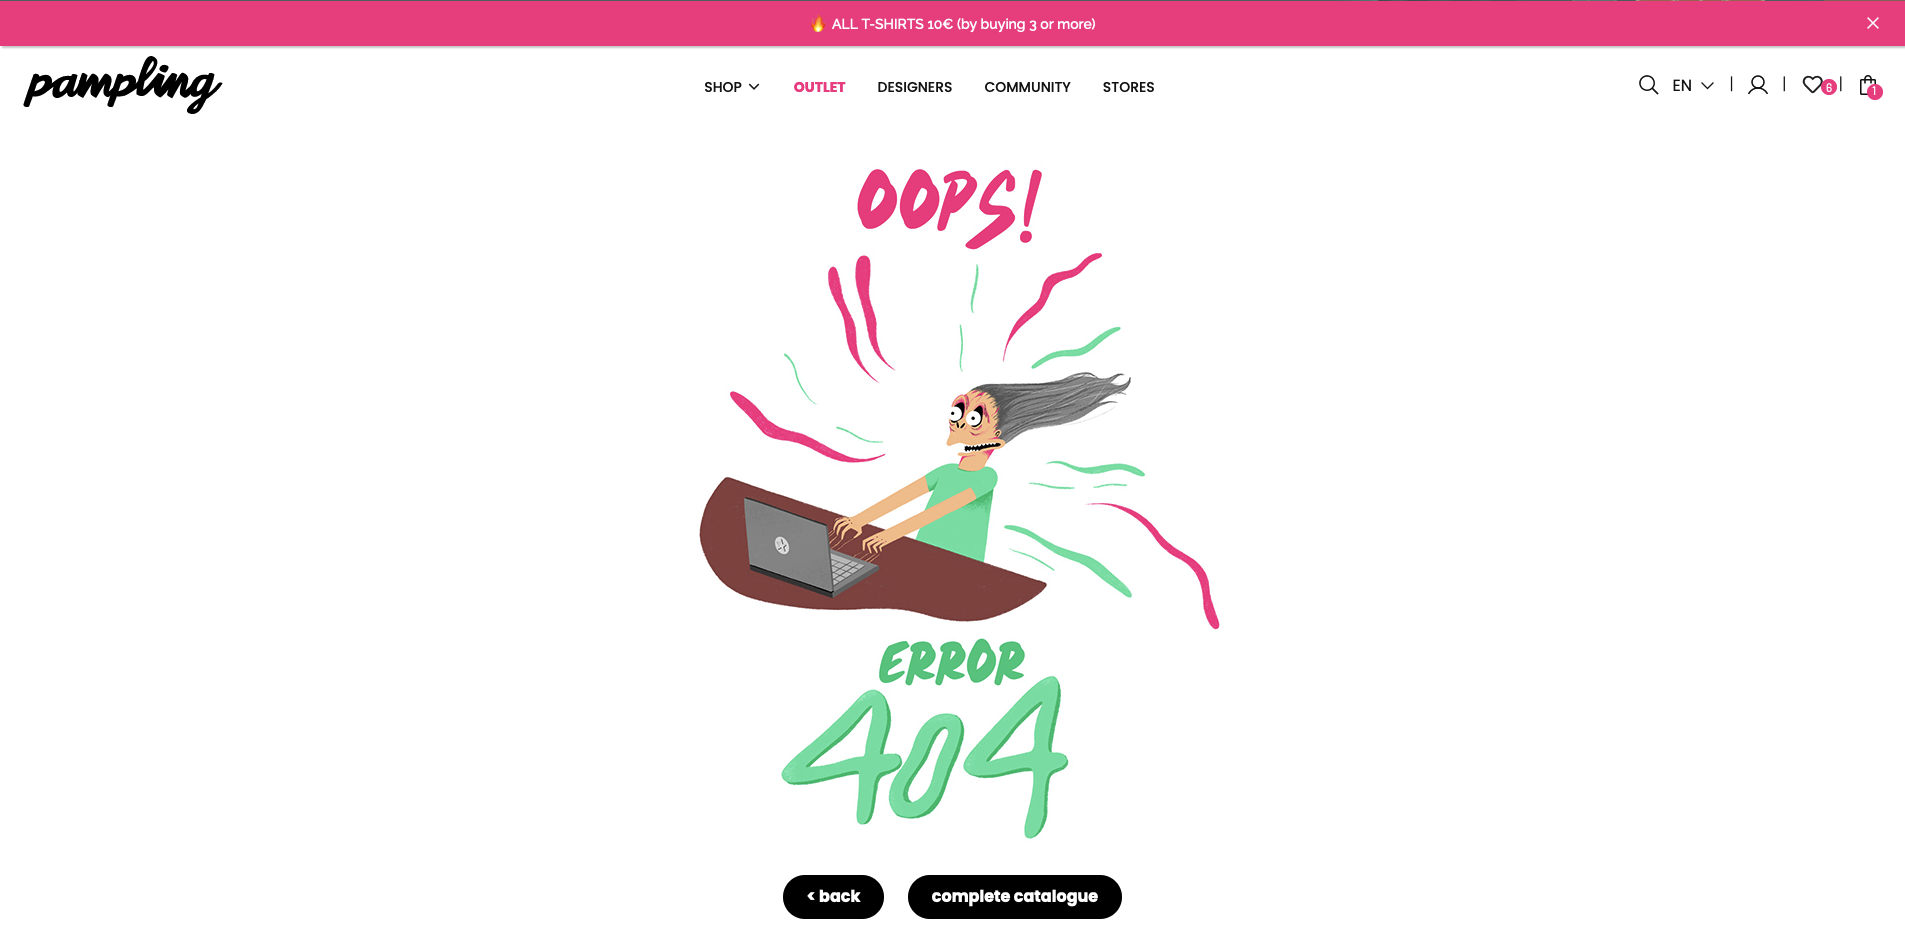
\includegraphics[scale=0.225]{images/404.png}
	\caption{404 webpage.}
	\label{fig:404}
\end{figure}
\subsection{404 Page}

A 404 HTTP error occurs when the webpage required is not available or it does not exist anymore. \\
The website's 404 page is not really well designed since it doesn't explain actually what happend but it just shows the
classic "Error 404" label, that for a common user doesn't mean anything.
Still, the menu bar on the top is still present and two buttons are shown to go back or to see the whole catalogue.
These are good choices in order to keep the user from losing context or be disoriented.

